\documentclass[tikz,border=3.14pt]{standalone}
\usepackage{tikz}
\usetikzlibrary{arrows.meta}
\usepackage{amsmath}
\usepackage{physics}

\ExplSyntaxOn
\msg_redirect_name:nnn { siunitx } { physics-pkg } { none }
\ExplSyntaxOff

\begin{document}
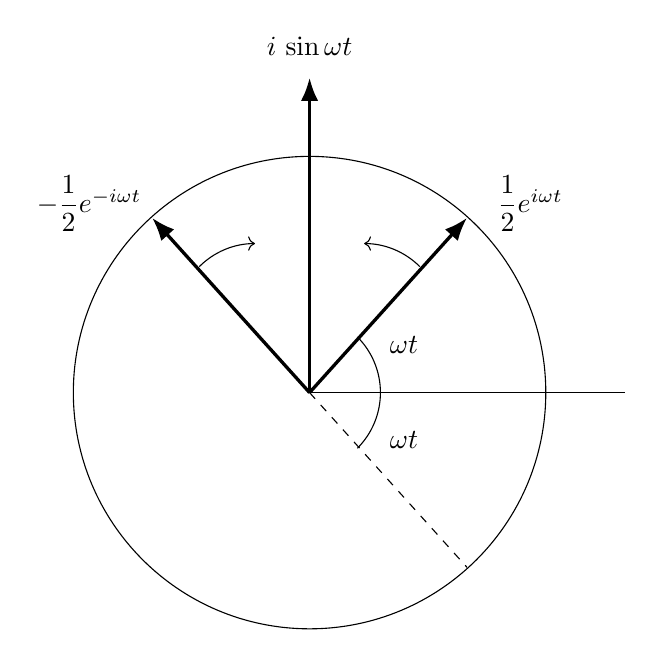
\begin{tikzpicture}[scale=2,
		vector/.style={-{Latex}, very thick}]

        \draw (0, 0) circle (1.5cm);

        \draw (0, 0) -- (2, 0);
        \draw [vector] (0, 0) -- (0, 2) node[pos=1.1] {$i \, \sin \omega t$};
        
        \draw [vector] (0, 0) -- (1, 1.11);
        \node at (1.4, 1.2) {$\dfrac{1}{2} e^{i \omega t}$};
        \draw (0.45, 0) arc(0:45:0.5);
        \node at (0.6, 0.3) {$\omega t$};

        \draw [vector] (0, 0) -- (-1, 1.11);
        \node at (-1.4, 1.2) {$-\dfrac{1}{2} e^{-i \omega t}$};

        \draw [dashed] (0, 0) -- (1, -1.11);
        \draw (0.45, 0) arc(0:-45:0.5);
        \node at (0.6, -0.3) {$\omega t$};

        \draw [->] (0.7, 0.8) arc (45:90:0.5);
        \draw [->] (-0.7, 0.8) arc (135:90:0.5);


\end{tikzpicture}
\end{document}